\documentclass{article}
%-------------------------------------------------------------------
% Paquetes necesarios
\usepackage[utf8]{inputenc} % Para caracteres especiales
\usepackage[spanish]{babel} % Para idioma español
\usepackage{amsmath, amssymb} % Para matemáticas
\usepackage{geometry} % Para ajustar márgenes 
\usepackage{graphicx} % Para agregar imágenes
\usepackage{float}
\usepackage{listings} % Para mostrar código
\usepackage{xcolor}   % Para colores
\definecolor{codegreen}{rgb}{0,0.6,0}
\definecolor{codegray}{rgb}{0.5,0.5,0.5}
\definecolor{codepurple}{rgb}{0.58,0,0.82}

% Configuración de estilo para Python
\lstdefinestyle{mystyle}{
    backgroundcolor=\color{white},   
    commentstyle=\color{codegreen},
    keywordstyle=\color{magenta},
    numberstyle=\tiny\color{codegray},
    stringstyle=\color{codepurple},
    basicstyle=\ttfamily\small,
    breakatwhitespace=false,         
    breaklines=true,                 
    captionpos=b,                    
    keepspaces=true,                 
    numbers=left,                    
    numbersep=5pt,                  
    showspaces=false,                
    showstringspaces=false,
    showtabs=false,                  
    tabsize=4,
    frame=single % Añade un marco alrededor
}

\lstset{style=mystyle}
%--------------------------------------------------------------------
% Inicio del documento
\begin{document}
%--------------------------------------------------------------------
% Portada
\begin{titlepage}
    
    \noindent % Evita la sangría inicial
    \begin{tabular}{@{}p{0.5\textwidth} p{0.5\textwidth}@{}}
        
\includegraphics[height=3cm, width=0.45\textwidth, keepaspectratio]{logos/uanl.png} & % Imagen izquierda
        \hfill 
\includegraphics[height=3cm, width=0.45\textwidth, keepaspectratio]{logos/fcfm.png} % Imagen derecha
    \end{tabular}
    
    \begin{center}
        \vspace*{2cm} % Espacio vertical
        \textbf{\Large Universidad Autónoma de Nuevo León} \\[2cm]
        
        \textbf{\Large Licenciatura en Ciencias Computacionales} \\[2cm]
        
        \textbf{\Large A10: Regresión Lineal Múltiple en Python} \\[2cm]
    
        \textbf{\large Materia: Inteligencia Artificial} \\[.5cm]
        \textbf{\large Maestro: Luis Ángel Gutiérrez Rodríguez} \\[2cm]
        
        \textbf{\large Rebeca Jaramillo Camarillo} \\[.5cm]
        \textbf{\large Matrícula: 2132988} \\[.5cm]
        \textbf{\large Grupo: 031} \\
        
        \vfill % Espacio vertical para ajustar el contenido al final de la página
        \textbf{\large Fecha: 23 de marzo de 2025} % Fecha automática
    \end{center}
	
\end{titlepage}

%--------------------------------------------------------------------
% Sección 1: Explique brevemente qué es la Regresión Lineal Múltiple y su significado.
\section{Introducción}
La regresión lineal múltiple es un modelo de regresión en cual se incluyen dos o más variables independientes. Es decir, la regresión lineal múltiple es un modelo estadístico que permite relacionar varias variables explicativas con una variable respuesta de manera lineal.\\
Por lo tanto, un modelo de regresión lineal múltiple sirve para encontrar una ecuación que relacione dos o más variables independientes con una variable dependiente. De forma que sustituyendo el valor de cada variable independiente se obtiene una aproximación del valor de la variable dependiente.\\

La fórmula de la regresión lineal se expresa matemáticamente como:
\begin{equation}
Y = b + m1X1 + m2X2 +…+ m(n)X(n)
\end{equation}
Donde Y es el resultado, X es la variable, m la pendiente (o coeficiente) de la recta y b la constante o también conocida como el “punto de corte con el eje Y” en la gráfica (cuando X=0)\\

En este documento, se presenta el paso a paso de una actividad de regresión lineal múltiple en Python para una mejor comprensión del tema.\\

%--------------------------------------------------------------------
% Metodología: Describe los pasos que tomaste para realizar la actividad, incluidos los fragmentos de código.
\section{Metodología}
A continuación, se muestran los pasos para resolver el ejercicio. Para ello, se usará de base el código realizado en la actividad 9 y simplemente se extenderá de 1 variable a 3 variables:

\subsection{Importar librerías, leer el archivo csv y cargarlo como un dataset de Pandas} 
\begin{lstlisting}[language=Python]
#Importar librerias necesarias
import numpy as np  
import pandas as pd  
import seaborn as sb 
import matplotlib.pyplot as plt 
from mpl_toolkits.mplot3d import Axes3D 
from matplotlib import cm 
plt.rcParams['figure.figsize'] = (16, 9)
plt.style.use('ggplot')
from sklearn import linear_model 
from sklearn.metrics import mean_squared_error, r2_score

#cargar los datos de entrada
data = pd.read_csv("./articulos_ml.csv")
\end{lstlisting}

\subsection{Filtrar datos y crear nueva variable}Para poder graficar en 3D se necesitan 2 variables. La primer variable seguirá siendo la cantidad de palabras y la segunda variable será la suma de 3 columnas de entrada: la cantidad de enlaces, comentarios y cantidad de imágenes.
\begin{lstlisting}[language=Python]
# Filtramos los datos como antes
filtered_data = data[(data['Word count'] <= 3500) & (data['# Shares'] <= 80000)]

# Creamos nueva variable combinando enlaces, comentarios e imagenes
suma = (filtered_data["# of Links"] + 
        filtered_data['# of comments'].fillna(0) + 
        filtered_data['# Images video'])
\end{lstlisting}

\subsection{Modelo de Regresión Lineal Múltiple}Se preparan los datos para regresión múltiple, luego se crea y se entrena el modelo. Finalmente, se hace la predicción.
\begin{lstlisting}[language=Python]
# Preparamos los datos para regresion multiple
dataX2 = pd.DataFrame()
dataX2["Word count"] = filtered_data["Word count"]
dataX2["suma"] = suma
XY_train = np.array(dataX2)  
z_train = filtered_data["# Shares"].values 

# Creamos un nuevo objeto de Regresion Lineal
regr2 = linear_model.LinearRegression()

# Entrenamos el modelo, esta vez, con 2 dimensiones obtendremos 2 coeficientes, para graficar un plano
regr2.fit(XY_train, z_train) 

# Hacemos predicciones con el modelo entrenado
z_pred = regr2.predict(XY_train)
\end{lstlisting}

\subsection{Evaluación del Modelo} 
\begin{lstlisting}[language=Python]
# Mostramos los resultados del modelo
# Los coeficientes
print("Coefficients: \n", regr2.coef_)
# Error cuadratico medio
print("Mean squared error: %.2f" % mean_squared_error(z_train, z_pred))
# Evaluamos el puntaje de varianza (siendo 1.0 el mejor posible)
print("Variance score: %.2f" % r2_score(z_train, z_pred))
\end{lstlisting}

\subsection{Visualización 3D del modelo}Se grafican las características de entrada en color azul y los puntos proyectados en el plano en rojo. Es importante recordar que en esta gráfica, el eje Z corresponde a la “altura” y representa la cantidad de Shares que se obtienen.
\begin{lstlisting}[language=Python]
# Visualizacion 3D del modelo
fig = plt.figure(figsize=(12, 8))
ax = fig.add_subplot(111, projection='3d')

# Creamos una malla, sobre la cual graficaremos el plano
xx, yy = np.meshgrid(np.linspace(0, 3500, num=10), np.linspace(0, 60, num=10))
 
# calculamos los valores del plano para los puntos x e y
nuevoX = (regr2.coef_[0] * xx)
nuevoY = (regr2.coef_[1] * yy)

# calculamos los correspondientes valores para z. Debemos sumar el punto de intercepcion
z = (nuevoX + nuevoY + regr2.intercept_)

# Graficamos el plano
ax.plot_surface(xx, yy, z, alpha=0.2, cmap='hot')

# Graficamos en azul los puntos en 3D
ax.scatter(XY_train[:, 0], XY_train[:, 1], z_train, c='blue', s=30, label='Datos reales')

# Graficamos en rojo las predicciones
ax.scatter(XY_train[:, 0], XY_train[:, 1], z_pred, c='red', s=40, label='Predicciones')

# Configuramos los ejes y la vista
ax.set_xlabel('Cantidad de Palabras')
ax.set_ylabel('Cantidad de Enlaces,Comentarios e Imagenes')
ax.set_zlabel('Compartido en Redes')
ax.set_title('Regresion Lineal con Multiples Variables')
ax.legend()

# Ajustamos la vista de la camara
ax.view_init(elev=30., azim=65)

# Mostramos el grafico
plt.show()
\end{lstlisting}

\subsection{Predicción}Si se quiere predecir cuántos "Shares" se obtienen para un artículo de 2000 palabras, 10 enlaces, 4 comentarios y 6 imágenes, se realiza lo siguiente:
\begin{lstlisting}[language=Python]
z_Dosmil = regr2.predict([[2000, 10+4+6]])
print("Prediccion de shares para articulo nuevo:", int(z_Dosmil))
\end{lstlisting}

\newpage
%--------------------------------------------------------------------
% Resultados: Presenta los resultados de tu análisis de Regresión Lineal Múltiple.
\section{Resultados}
A continuación, se presentan los resultados del análisis de Regresión Lineal Múltiple\\

Visualización 3D del modelo de regresión:
\begin{figure}[H]
    \centering
    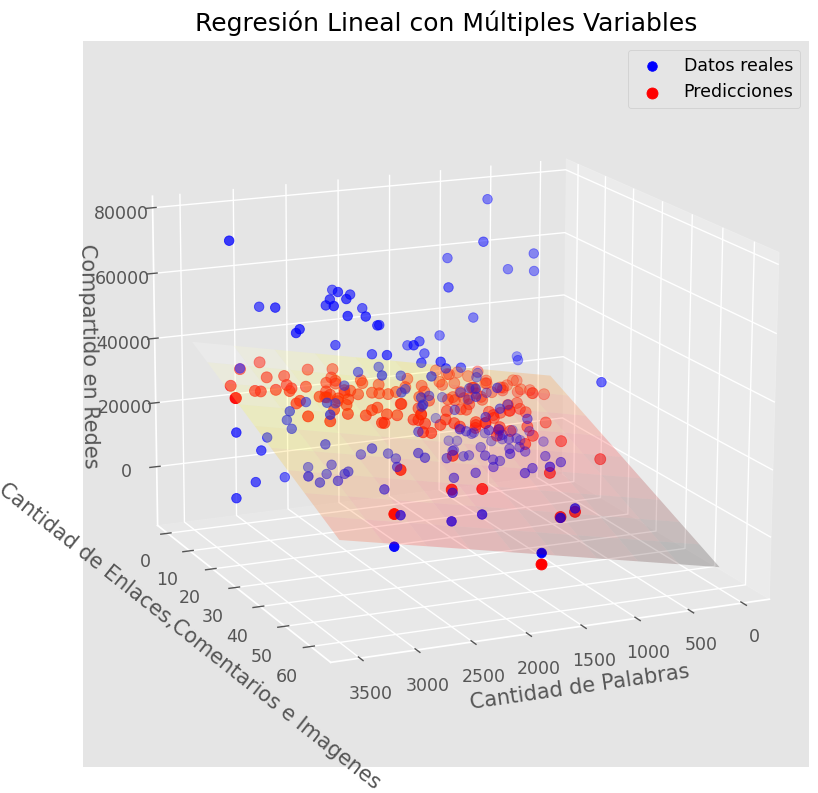
\includegraphics[width=1\linewidth]{img/a10_modelo3D.png}
    \caption{Modelo 3D. Paso 5}
    \label{fig:figure2}
\end{figure}

\newpage

Como vemos, obtenemos 2 coeficientes (cada uno correspondiente a las 2 variables predictivas), por lo que al graficar será plano en 3 Dimensiones en lugar de una linea. El error obtenido es grande, mejor que el obtenido en la regresión lineal, y el puntaje de Varianza mejora casi el doble del anterior (aunque sigue siendo muy malo, muy lejos del 1).
\begin{figure}[H]
    \centering
    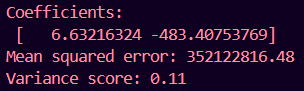
\includegraphics[width=0.5\linewidth]{img/a10_ecuacion.png}
    \caption{Resultados del modelo. Paso 4}
    \label{fig:figure2}
\end{figure}

El resultado de la predicción para un artículo de 2000 palabras, 10 enlaces, 4 comentarios y 6 imágenes es de 20,518 "shares":
\begin{figure}[H]
    \centering
    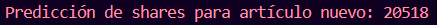
\includegraphics[width=0.7\linewidth]{img/a10_prediccion.png}
    \caption{Predicción. Paso 6}
    \label{fig:figure2}
\end{figure}

%--------------------------------------------------------------------
% Conclusión: Resume tus hallazgos y cualquier información obtenida de la actividad.
\section{Conclusión}
Aunque la aplicación de esta actividad mostró los resultados esperados(coeficientes, error cuadrático medio y puntaje de varianza), es importante recordar que esto fue principalmente con fines de aprendizaje. En la práctica, para obtener predicciones más precisas, es necesario utilizar un mayor número de variables y asegurarse de que éstas sean relevantes.
%--------------------------------------------------------------------
% Fin del documento
\end{document}